\documentclass{article}
\title{Maximum depositional age estimation revisited}
\author{Pieter Vermeesch\\
  University College London\\
  \texttt{p.vermeesch@ucl.ac.uk}
}
\date{August 20, 2020}
\usepackage{natbib,fullpage,graphicx,caption,lineno,setspace,upquote}
\begin{document}

%\onehalfspace

%\linenumbers

\maketitle

\begin{abstract}
  In a recent review published in this journal, Coutts et al.  (2019,
  \textit{Geoscience Frontiers}, 10, 4, 1421--1435) compared nine
  different ways to estimate the maximum depositional age (MDA) of
  siliclastic rocks by means of detrital geochronology.  Their results
  show that among these methods three are positively and six
  negatively biased. This paper investigates the cause of these biases
  and proposes a solution to it.  A simple toy example shows that it
  is theoretically impossible for the reviewed methods to find the
  correct depositional age in even a best case scenario: the MDA
  estimates drift to ever smaller values with increasing sample
  size. This issue can be solved using a maximum likelihood model that
  was originally developed for fission track thermochronology by
  Galbraith and Laslett (1993, \textit{Nucl. Tracks Rad. Meas.}, 21,
  4, 459--470).  This approach parameterises the MDA estimation
  problem with a binary mixture of discrete and continuous
  distributions. The `Maximum Likelihood Age' (MLA) algorithm
  converges to a unique MDA value, unlike the ad hoc methods reviewed
  by Coutts et al. (2019). It successfully recovers the depositional
  age for the toy example, and produces sensible results for realistic
  distributions. This is illustrated with an application to a
  published dataset of 13 sandstone samples that were analysed by both
  LA-ICPMS and CA-TIMS U--Pb geochronology. The ad hoc algorithms
  produce unrealistic MDA estimates that are systematically younger
  for the LA-ICPMS data than for the CA-TIMS data. The MLA algorithm
  does not suffer from this negative bias. The MLA method is a purely
  statistical approach to MDA estimation. Like the ad hoc methods, it
  does not readily accommodate geological complications such as
  post-depositional Pb-loss, or analytical issues causing erroneously
  young outliers. The best approach in such complex cases is to
  re-analyse the youngest grains using more accurate dating
  techniques.  The results of the MLA method are best visualised on
  radial plots. Both the model and the plots have applications outside
  detrital geochronology, for example to determine volcanic eruption
  ages.
\end{abstract}

\begin{center}
  keywords: zircon; U-Pb; geochronology; statistics; maximum depositional age
\end{center}

\section{Introduction}

Detrital geochronology is often the only way to estimate the
depositional age of siliclastic rocks in the absence of fossils or
volcanic ash layers. Detrital zircon U--Pb geochronology in particular
has become a popular technique to obtain maximum depositional ages
(MDAs). Numerous MDA estimation algorithms have been proposed over the
years \citep{nelson2001, barbeau2009, dickinson2009, tucker2013,
  chen2016, zhang2016, ross2017, herriott2019, copeland2020}. In a
detailed review paper that was recently published in this journal,
\citet{coutts2019} compared and contrasted the most popular among
these methods, namely:

\begin{enumerate}
\item the youngest single grain (YSG);
\item the mode of the youngest graphical peak on a probability density
  plot (YPP);
\item the youngest grain cluster at $1\sigma$ (YGC1$\sigma$) or
  $2\sigma$ (YGC2$\sigma$);
\item the youngest detrital zircon estimated by \citet{ludwig2003}'s
  Monte Carlo resampling algorithm (YDZ);
\item the outcome of \citet{ludwig2002}'s TuffZirc algorithm;
\item the weighted mean of the youngest three (Y3Z) or four (Y4Z)
  zircons;
\item the weighted mean of the grains in the youngest peak of a
  probability density plot ($\tau$); and
\item the minimum age of grains selected by \citet{gehrels2003}'s
  AgePick algorithm.
\end{enumerate}

\noindent Additionally, they also introduced a new estimator:

\begin{enumerate}
  \setcounter{enumi}{8}
\item the `Youngest Statistical Population' (YSP), which groups the
  youngest sub-sample of more than two grains that pass a Chi-square
  test for homogeneity.
\end{enumerate}

Using numerical simulations and synthetic age distributions,
\citet{coutts2019} found that all but three of these methods gradually
drift to younger ages with increasing sample size.  The only
exceptions were the YPP, $\tau$ and YSP methods, which converged to
ages that were systematically too old. The failure of YPP and $\tau$
to retrieve the correct depositional age reflects the underlying flaws
of the probability density plots (PDPs) on which they are based. The
shortcomings of PDPs are explained in detail by \citet{vermeesch2012b}
and \citet{vermeesch2018b} and won't be discussed further in this
paper. The positive bias of the YSP method will be briefly discussed
in Section~\ref{sec:discussion}. The remainder of the paper will focus
on the undesirable drift of the remaining six MDA estimation
algorithms towards geologically unreasonable young values.\\

Section~\ref{sec:convergence} will prove that it is theoretically
impossible for the YSG, YGC1$\sigma$/2$\sigma$, YDZ and Y3Z/Y4Z
methods to converge to the correct solution even in a best case
scenario. Section~\ref{sec:galbraith} shows that the `minimum age
model' of \citet{galbraith1993} does not suffer from this
problem. This maximum likelihood based method was developed for
detrital fission track thermochronology but can be equally useful for
zircon U--Pb studies in a modified form developed by
\citet[][p.107]{galbraith2005}. We will refer to the minimum age model
as the `maximum likelihood age' (MLA) method to avoid confusion with
minimum depositional age estimation, which is an entirely different
subject.\\

Section~\ref{sec:examples} applies the MLA algorithm to a detrital
zircon U--Pb dataset from the Colorado Plateau Coring Project. This
case study validates the different MDA methods by comparing
measurements obtained by Laser Ablation Inductively Coupled Plasma
Mass Spectrometry (LA-ICPMS) with measurements obtained on the same
samples by Chemical Abrasion Thermal Ionisation Mass Spectrometry
(CA-TIMS). The new MLA algorithm is the only method that passes this
stringent test.\\

Despite the advantages of the MLA method over all existing MDA
estimation algorithms, it is not a silver bullet for samples that have
a fat tail at the young end of the age spectrum, or that have been
affected by post-depositional Pb-loss. Section~\ref{sec:limitations}
discusses these limitations and provides suggestions to mitigate their
effects.

\section{On the failure of existing MDA algorithms to converge}
\label{sec:convergence}

The YSG, YGC1$\sigma$/2$\sigma$, YDZ and Y3Z/Y4Z methods essentially
amount to averaging the $n$ youngest grains obtained by some selection
criterion. The selection criterion can be simple (e.g., YSG) or
complex (YDZ).  But all these algorithms boil down to analysing the
young tails of detrital age spectra. This is a difficult thing to do
with ad hoc methods.\\

Detrital age spectra are the convolution of two probability
distributions: (1) the distribution of the true (but unknown) zircon
U--Pb ages; and (2) the distribution of their analytical
errors. Analytical uncertainty obscures the true ages and must be
accounted for during MDA estimation.  Geochronologists generally make
the reasonable assumption that the analytical errors follow a normal
distribution with mean $\mu = 0$ and standard deviation
$\sigma$. Under this condition it is well known that the actual U--Pb
age is approximately 95\% likely to fall in a $\pm$2$\sigma$ interval
around the measured value. However this is only true when considering
a single analysis.\\

When multiple measurements are considered together, then the
likelihood that the measured value is more than $\pm$2$\sigma$ away
from the true value increases. In statistics this is known as a
`Type-1 error'. As the number of analyses increases, so does the
probability that at least one value falls outside the $\pm$2$\sigma$
interval. Given a sufficiently large sample size, there inevitably
comes a point when the data contain values that differ from the true
value by 3$\sigma$ or more. This is true for both tails of the normal
distribution. In the context of MDA estimation, it means that the
youngest date in a huge sample may be less than the actual
depositional age.\\

To further explore this important point, let us consider the simplest
case of an MDA estimation exercise. Suppose that 100\% of the grains
in a sample are concordant and syn-depositional at 10~Ma, with
normally distributed uncertainties of 1~Ma at 1$\sigma$. The solution
to this toy example is trivial. The depositional age is simply given
by the mean of all the dates. Yet six of the nine MDA estimation
algorithms reviewed by \citet{coutts2019} fail to retrieve it (YPP,
$\tau$ and YSP don't, but will fail in nearly all non-trivial
examples).\\

\begin{figure}[!ht]
  \centering \includegraphics[width=.6\textwidth]{youngestN.pdf}
  \parbox{.6\textwidth}{
    \caption{Exact quantiles of a normal distribution with 10~Ma mean and
      1~Ma standard deviation. The step functions show the expected age of
      the $n$\textsuperscript{th} youngest grain (for $1 \leq n \leq 10$)
      in a sample of $N$ grains (for $1 \leq N \leq 50$). All these
      functions monotonically decrease with increasing sample size. This
      means that any MDA estimation algorithm that is based on the
      $n$\textsuperscript{th} youngest grain(s), or averages thereof, can
      never converge to the true depositional age.}
    \label{fig:youngestN}
  }
\end{figure}

Figure~\ref{fig:youngestN} shows why existing MDA estimation methods
fail the toy example. It plots the expected age\footnote{The expected
  age is given by $\mu + \sigma\sqrt{2} \mbox{erf}^{-1} \left[2 n/N -
    1\right]$, where erf\textsuperscript{-1} is the inverse error
  function.} of the $n$\textsuperscript{th} youngest grain among a
sample of $N$ grains drawn from our normal distribution with mean $\mu
= 10$ and standard deviation $\sigma = 1$.  For example, consider a
sample containing $N = 5$ grains, then the expected age of the
youngest grain ($n = 1$) is the 1/5\textsuperscript{th} quantile of
the normal distribution, which is 9.16~Ma. When the sample size is
increased to 20 grains, then the expected value for the youngest age
is given by the 1/20\textsuperscript{th} quantile, which is 8.36~Ma.\\

Thus, the youngest single grain age monotonically decreases with
increasing sample size, and so does the second youngest grain ($n =
2$), the third youngest grain ($n = 3$) and so forth. Also the average
of the youngest $n$ grains decreases with increasing sample size, and
all the other grain selection criteria do so as well. The failure of
existing MDA estimation algorithms to solve the simplest toy example
undermines their credibility in more complex scenarios.

\section{The maximum likelihood model of \citet{galbraith1993}}
\label{sec:galbraith}

\begin{figure}[!ht]
  \centering
  \includegraphics[width=.8\textwidth]{Galbraith.pdf}
  \parbox{.8\textwidth}{
    \caption{Schematic illustration of the four parameter minimum age
      model (left) and its three parameter special case (right). The
      minimum age is marked by $t_m$. Redrafted from Figure~6.3 of
      \citet{galbraith2005}.}
    \label{fig:galbraith}
  }
\end{figure}

The failure of existing MDA estimation algorithms to find the correct
solution for the toy example is diagnostic of the fact that they are
ad hoc algorithms that lack a formal statistical basis. It is
desirable for statistical estimation techniques to converge to the
true solution with increasing sample size. Unfortunately none of the
existing method manage to do so. The conventional way to solve this
issue is to parameterise the problem and determine the parameters by
Maximum Likelihood Estimation (MLE). Geological examples of this
approach include isochron regression
\citep{titterington1979,york2004}, concordia age estimation
\citep{ludwig1998} and finite mixture modelling
\citep{galbraith1990b,sambridge1994}. The MLE approach can also be
used for MDA estimation. In fact, such an algorithm already exists.\\

\citet{galbraith1993} introduced a minimum age estimator for fission
track thermochronology that is equally applicable to U--Pb
geochronology. The model asumes that the data were drawn from a two
component mixture, in which a fraction $\pi_\gamma$ of the population
is derived from a discrete minimum age peak at $t_m = \exp[\gamma]$
and the remaining fraction $(1 - \pi_\gamma)$ of the grains were drawn
from a (log)normal distribution with location parameter $\mu$ and
dispersion parameter $\sigma$, truncated at $t_m$
(Figure~\ref{fig:galbraith}). The four model parameters ($\gamma$,
$\pi_\gamma$, $\mu$ and $\sigma$) can be estimated by maximising the
likelihood function using an appropriate error model for the
analytical uncertainties.\\

The original fission track implementation of \citet{galbraith1993}'s
maximum likelihood model assumed binomial counting errors
\citep{touw1997}.  An alternative formulation using normal errors was
formulated by \citet[][p.107]{galbraith2005}. This version of the
model is most appropriate for MDA estimation by detrital U--Pb
geochronology. The minimum age model will be referred to as the MLA
(Maximum Likelihood Age) method in the remainder of this paper, so as
to avoid any confusion with minimum depositional age estimation.\\

Standard MLE theory also provides a way to estimate the uncertainties
of the model parameters. This is done by inverting the negative matrix
of second derivatives (i.e. the Hessian) of the log-likelihood
function with respect to the parameters. Experience shows that the
uncertainties of $\gamma$ and $\pi_\gamma$ are generally smaller than
those of $\mu$ and $\sigma$. Because $\mu$ and $\sigma$ are not
directly relevant to the MDA estimation problem anyway, there is
little harm in reducing the number of model parameters from four to
three, by requiring that $\gamma = \mu$. The resulting gain in
numerical stability benefits small datasets whilst having only a minor
effect on the accuracy of the MDA estimates.\\

It can be shown that among all statistical estimators, the MLE
approach is the most \emph{efficient}, which means that it yields the
most precise estimates for any given sample size. MLE algorithms are
also \emph{consistent}, which means that they are guaranteed to
converge to the true solution with increasing data size (assuming that
the model assumptions are met). Thus the MLA method fixes the key
issue with existing MDA estimation methods. Applying it to the toy
example asymptotically yields parameter values of $\pi_\gamma = 1$,
$\sigma = 0$ and $\gamma = 2.3$, which corresponds to the correct
answer of $t_m = 10$~Ma.

\section{Application to U--Pb data from the Colorado Plateau}
\label{sec:examples}

\begin{figure}[!ht]
  \centering
  \includegraphics[width=.9\textwidth]{297.pdf}
  \parbox{.9\textwidth}{
    \caption{Radial plots and MLA estimates for sample 297 of
      \citet[][LA-ICPMS data, left]{gehrels2020} and \citet[][CA-TIMS
        data, right]{rasmussen2020}, calculated with \texttt{IsoplotR}
      \citep{vermeesch2018b}.  Uncertainty estimates are reported as
      studentised 95\% confidence intervals. Both datasets are
      overdispersed with respect to the analytical uncertainties. The
      MLA estimates agree to within 0.6\% despite the great differences
      in sample size and analytical precision between the two
      datasets. Existing ad hoc MDA estimation algorithms do not fare so
      well, resulting in differences of 2 -- 17\% between the LA-ICPMS
      and CA-TIMS data.}
    \label{fig:297}
  }
\end{figure}

Leaving the toy example behind and moving on to a geologically more
realistic example, we will now apply the MLA model to a recently
published dataset of detrital zircon U--Pb ages obtained from the
Colorado Plateau Coring Project (CPCP). The dataset contains 13
detrital zircon samples that were extracted from a $\sim$520~m drill
core in Petrified Forest National Park (Arizona, USA).\\

The 13 samples belong to the Permo-Triassic Coconino, Moenkopi and
Chinle Formations.  Between 221 and 308 randomly selected zircon
grains from each sample were dated by LA-ICPMS, yielding 13 U--Pb age
spectra ranging from 189 to 3428~Ma \citep{gehrels2020}. Subsequently,
the youngest 2 -- 19 grains from each sample were extracted from the
LA-ICPMS grain mount and re-analysed by high precision CA-TIMS
\citep{rasmussen2020}.  This paired LA-ICPMS + CA-TIMS dataset allows
us to compare the performance of the different MDA estimators across a
range of sample sizes and analytical precision.\\

Figure~\ref{fig:297} shows the LA-ICPMS and CA-TIMS age estimates for
sample 297 on so-called radial plots. These are a graphical device
that was invented by Rex Galbraith, the creator of the MLA model
\citep{galbraith1988, galbraith1990a}. The radial plot is designed to
visualise heteroscedastic datasets (i.e., datasets with unequal
uncertainties).  It is the most elegant way to visualise the results
of the MLA model, which explicitly takes into account this
heterescedasticity. See the Appendix for further details.\\

The LA-ICPMS data of sample 297 follow a bimodal age distribution.
This is evident in Figure~\ref{fig:297} as two linear arrays on the
radial plot radiating from the origin towards the radial scale at
$\sim$220~Ma and $\sim$1800~Ma, respectively. Unsurprisingly, the
radial plot of the CA-TIMS data looks very different. It exhibits a
unimodal distribution with ages ranging from 220 to 226Ma.\\

From the radial plots it is evident that age dispersion exceeds
analytical uncertainty for both the LA-ICPMS and CA-TIMS datasets. In
fact none of the 13 samples pass a Chi-square test for age
homogeneity, indicating the presence of geological dispersion.  The
overdispersion of the LA-ICPMS data is expected because these were
meant to capture multiple provenance components. However the excess
scatter of the CA-TIMS data merits further discussion.\\

The overdispersion of the CA-TIMS data could either reflect the
presence of multiple detrital components of similar age, or it could
be caused by protracted pre-eruptive residence of zircon in a volcanic
magma chamber.  In either case, the CA-TIMS data present a similar
statistical challenge as the LA-ICPMS data in that it is not
immediately obvious how to estimate the MDA.\\

To meet this challenge, all the MDA estimate algorithms were applied
to both the LA-ICPMS and CA-TIMS datasets. Thus we can objectively
compare the effects of the different algorithms and of the different
analytical techniques (Section~\ref{sec:comparison}).

\section{Empirical comparison of the different MDA algorithms}
\label{sec:comparison}

\begin{figure}[!ht]
  \includegraphics[width=\textwidth]{TIMSvsICP.pdf}
  \caption{Pairwise comparison of the 13 LA-ICPMS and CA-TIMS datasets
    using 12 different MDA estimators. Error bars are shown at 95\%
    confidence.  The area above the 1:1 line represents a `forbidden
    zone' where the CA-TIMS estimates exceed the LA-ICPMS
    estimates. The MLA algorithm is the only method that does not
    suffer from this problem. It is the only algorithm that provides
    reasonable MDA values for all samples.}
  \label{fig:TIMSvsICP}
\end{figure}

Both radial plots and MLA calculations were made in
\citet[\texttt{IsoplotR},][]{vermeesch2018c}. See Appendix~B for
further details.\\

Applying the MLA method to sample 297 yields MDA estimates of
219.68$\pm$0.46~Ma and 221.09$\pm$0.99~Ma for the LA-ICPMS and CA-TIMS
data, respectively. The small (-0.6\%) age difference between the two
estimates contrasts starkly with existing methods such as YSG
(-17.4\%), YGC1$\sigma$ (-5.4\%), YGC2$\sigma$ (-4.5\%), Y3Z (-7.8\%),
Y4Z (-5.2\%), YDZ (-17.5\%) and YSP (-2.1\%). Repeating the same
exercise for the remaining 12 samples confirms this picture.\\

Figure~\ref{fig:TIMSvsICP} compares the MDA estimates of the LA-ICPMS
and CA-TIMS data for all the methods discussed in this paper.  The
results are shown as bivariate scatter plots with 95\% confidence
intervals shown as error bars. These plots can be divided into three
zones.

\begin{enumerate}
\item The 1:1 line marks samples whose LA-ICPMS and CA-TIMS based MDA
  estimates agree within error. This is the expected scenario for
  compositionally homogenous zircon crystals without common Pb.
\item The area below the 1:1 line groups LA-ICPMS based MDA estimates
  that are older than their CA-TIMS based counterparts. This may
  indicate complications such as common Pb or the presence of small
  scale growth zones.
\item The area above the 1:1 line is a `forbidden zone'. In general,
  one would not expect CA-TIMS ages to exceed the corresponding
  LA-ICPMS ages, unless the zircons have experienced post-depositional
  Pb-loss. It is unlikely that such Pb-loss is a common occurence in
  nature, for reasons that will be discussed in
  Section~\ref{sec:limitations}.
\end{enumerate}

All but two of the ten ad hoc MDA estimation methods shown on
Figure~\ref{fig:TIMSvsICP} spill over into the `forbidden zone'.  The
YSG, YGC1$\sigma$, YGC2$\sigma$, Y3Z, Y4Z and YDZ methods are the
worst offenders because all their LA-ICPMS based MDA estimates are
younger than their CA-TIMS based MDA estimates. This troubling result
is likely caused by the sample-size effect discussed in
Section~\ref{sec:convergence}: because the LA-ICPMS datasets are two
orders of magnitude larger than the CA-TIMS datasets, they are much
more likely to drift towards unreasonably young values.\\

The MLA method does not suffer from this problem. All its MDA
estimates either fall on or below the 1:1 line. The only two ad hoc
methods that fare reasonably well are YPP and TuffZirc.  However the
YPP method does not provide a measure of uncertainty, while the
TuffZircon dates include one sample in the forbidden zone and one
sample whose LA-ICPMS age is three times older than the CA-TIMS
age. All things considered, the MLA method provides the most sensible
results.\\

The first two panels of Figure~\ref{fig:TIMSvsICP} show the results of
the 3-parameter and 4-parameter versions of the MLA algorithm,
respectively.  The difference between the two models is negligible
($\ll$1\%), reflecting the insensitivity of the method to the
parametric model assumptions.

\section{Limitations}
\label{sec:limitations}

Any statistical model is only as good as the assumptions that it
makes. For the minimum age model, these assumptions are that

\begin{enumerate}
\item the true age distribution approximately follows the functional
  form shown in Figure~\ref{fig:galbraith}; and
\item the analytical uncertainties are well characterised.
\end{enumerate}

The first assumption is generally easy to verify. If the young end of
the age spectrum is marked by a cluster of nearly concordant ages,
then the minimum age model will appropriately average these. And it
will do so even if the old end of the spectrum does not look like a
(log)normal distribution. It is not uncommon for detrital zircon U--Pb
age distributions to be fat tailed at both ends of the
spectrum. However, the similar results obtained by the 3- and
4-parameter formulations of the MLA algorithm indicates that this is
generally not a problem.\\

If the age difference between the youngest and the second youngest
grains in a sample is significantly greater than their respective
analytical uncertainties, then the minimum age model will simply
return the youngest age as a result. In other words, for fat tailed
age spectra, the minimum age model reduces to the YSG model. This is
the most sensible solution from a statistical point of view. In the
absence of a discrete youngest age peak, the objections to the YSG
model raised in Section~\ref{sec:convergence} and
Figure~\ref{fig:youngestN} do not apply. However whether age of the
youngest grain is also the most sensible solution from a geological
point of view is a different matter.\\

Post-depositional Pb-loss is one way to violate assumption~2. Zircon
grains that have experienced Pb-loss can yield precise yet inaccurate
U--Pb age estimates that plot in the `forbidden zone' of the LA-ICPMS
vs. CA-TIMS plot (Section~\ref{sec:comparison}). The minimum age model
is unable to detect this problem. But neither, of course, are any of
the existing MDA estimation algorithms. In the absence of a
statistically sound solution, it is useful to inspect any textural or
compositional data for clues to identify grains that have been
affected by Pb-loss. For example, if the young outliers are all
characterised by extremely high U- and/or Th-concentrations, then this
could be taken as evidence for radiation damage induced Pb-loss. Such
additional information can be visualised on the radial plot as
optional fill colours.\\

However, given the low diffusivity of Pb in zircon at the temperatures
found in most sedimentary basins, post-depositional Pb-loss is
probably unlikely to be a common problem in detrital geochronology
\citep{cherniak2001, copeland2020}. It is possible that many
anomalously young ages that have been attributed to common Pb-loss to
are instead just ordinary outliers violating assumption~2. The
probability that a dataset contains such anomalously young values
increases with sample size. In principle these values could be removed
by outlier detection algorithms. But all such algorithms are heuristic
by nature and are not guaranteed to produce sensible results.\\

A better albeit more onerous solution for fat tailed age distributions
is to re-analyse the youngest grains either by internal isochron
analysis \citep{nemchin2005}, or by CA-TIMS geochronology as shown in
this paper. After such validation, even a single isolated grain of
zircon can provide a robust MDA constraint.

\section{Discussion}
\label{sec:discussion}

This paper has shown that the MLA model of \citet{galbraith1993} and
\citet{galbraith2005} is superior to all the MDA estimation algorithms
reviewed by \citet{coutts2019}. It is the only method that is built on
solid statistical foundations, and the only method that can converge
to the correct solution with increasing sample size. In the absence of
complications with recent Pb-loss or young outliers, the MLA method is
entirely objective and completely hands off. It does not require any
arbitrary decision such as the number of grains to average (Y3Z, Y4Z),
or the probability cutoff to use (YGC1$\sigma$, YGC2$\sigma$).\\

Although this objectivity is appealing in several ways, it lacks any
geological context. \citet{copeland2020} argues that detrital zircon
grains cannot be grouped into discrete (maximum depositional) age
components without additional geochemical justification. However
whilst it is true that MLA estimates may not correspond to a
particular geological event, it should be emphasised that they are not
meant to do so.  The principal purpose of any MDA algorithm is to
obtain an upper limit for the depositional age. Whether this upper
limit corresponds to a particular geological event, or to a mixture of
multiple overlapping events, is a different issue.\\

At first glance, the MLA model may seem similar to
\citet{coutts2019}'s YSP method, because both algorithms assume that
the minimum age belongs to a discrete age component. However there is
a crucial difference between the two techniques. The YSP method
assumes that it is possible to make a clean separation between grains
whose true ages belong to the youngest age peak, and grains whose true
ages belong to older age components.  In reality this distinction is
blurred by the analytical uncertainties. The rank order of single
grain age \emph{estimates} may not necessarily be the same as that of
the \emph{true} U--Pb ages. This makes the YSP method biased relative
to the minimum age model.  The latter does not arbitrarily assign the
grains to two groups, but jointly considers all the age estimates when
fitting the model parameters.\\

Besides its applications in fission track thermochronology and
detrital geochronology, the MLA model can be used in other Earth
Science applications as well, such as the determination of eruption
ages from collections of volcanic zircon ages. Volcanic rocks often
exhibit positively skewed age distributions with a short tail of
syn-eruptive U--Pb ages and a long tail of pre-eruptive or xenocrystic
ages. In this context the MLA model would be a good alternative to ad
hoc approaches such as YSG and YSP that have previously been used, or
to the more sophisticated Bayesian approaches that have recently been
proposed \citep{keller2018}. It would also be useful to visualise such
volcanic datasets on radial plots instead of the interval plots that
are currently used.

\section{Acknowledgments}

P.V. would like to thank George Gehrels, Peter Copeland and Daniel
Coutts for constructive reviews that significantly improved the
paper. This research was supported by NERC standard grant
\#NE/T001518/1 (`Beyond Isoplot').

\section*{Appendix~A: about radial plots}

Like the MLA model itself, radial plots were originally developed by
Rex \citet{galbraith1988,galbraith2005} for the purpose fission track
geochronology. And like the MLA model, radial plots can be equally
useful for U--Pb and other geochronometers
\citep{vermeesch2009c,vermeesch2018c}. Let $z_j$ and $s_j$ be the
log-transformed values of $N$ single grain ages $t_j$ and their
standard errors $\sigma_j$ (for $1 \leq j \leq N$):

\begin{equation}
  z_j = \log(t_j) \mbox{~and~} s_j = \sigma_j/t_j
\end{equation}

\noindent then a radial plot is a bivariate $(x_j,y_j)$ scatterplot
with:

\begin{equation}
  x_j = 1/s_j \mbox{~and~} y_j = (z_j - z_\circ)/s_j
\end{equation}

\noindent where $z_\circ$ is a reference value such as the weighted
mean of the $z_j$ values. Radial plots allow the observer to
simultaneously assess both the magnitude and the precision of
quantitative data. Each point on the diagram represents a single grain
analysis. Old grains plot at high (positive) angles to the origin,
whereas young grains plot at low (negative) angles.  The analytical
uncertainty can be obtained by extrapolating lines from the origin to
the radial scale through the top and the bottom of an imaginary
2$\sigma$-error bar added to each sample point. Thus, precise
measurements plot towards the right hand side of the diagram, whereas
imprecise measurements plot towards the left.  Drawing two parallel
lines at 2$\sigma$ distances from either side of the origin allow the
analyst to visually assess whether all the single grain ages within a
sample agree within the analytical uncertainties.\\

With its ability to visualise heteroscedastic datasets (i.e., datasets
with unequal uncertainties), the radial plot realises the unfulfilled
promise of the probability density plot \citep{vermeesch2012b}.  It is
the most elegant way to visualise the results of the MLA model, which
explicitly takes into account this heterescedasticity.  Discrete
components (including despositional age components) in a mixed age
distribution can be easily spotted as linear arrays radiating from the
origin towards the radial scale (left panel of
Figure~\ref{fig:297}). Radial plots and the MLA model have been
implemented in \texttt{Java}
\citep[\texttt{RadialPlotter},][]{vermeesch2009c} and \texttt{R}
\citep[\texttt{IsoplotR},][]{vermeesch2018c}. Detailed instructions
for the latter application are provided in Appendix~B.

\section*{Appendix~B: Implementation in \texttt{IsoplotR}}

\begin{figure}[!ht]
  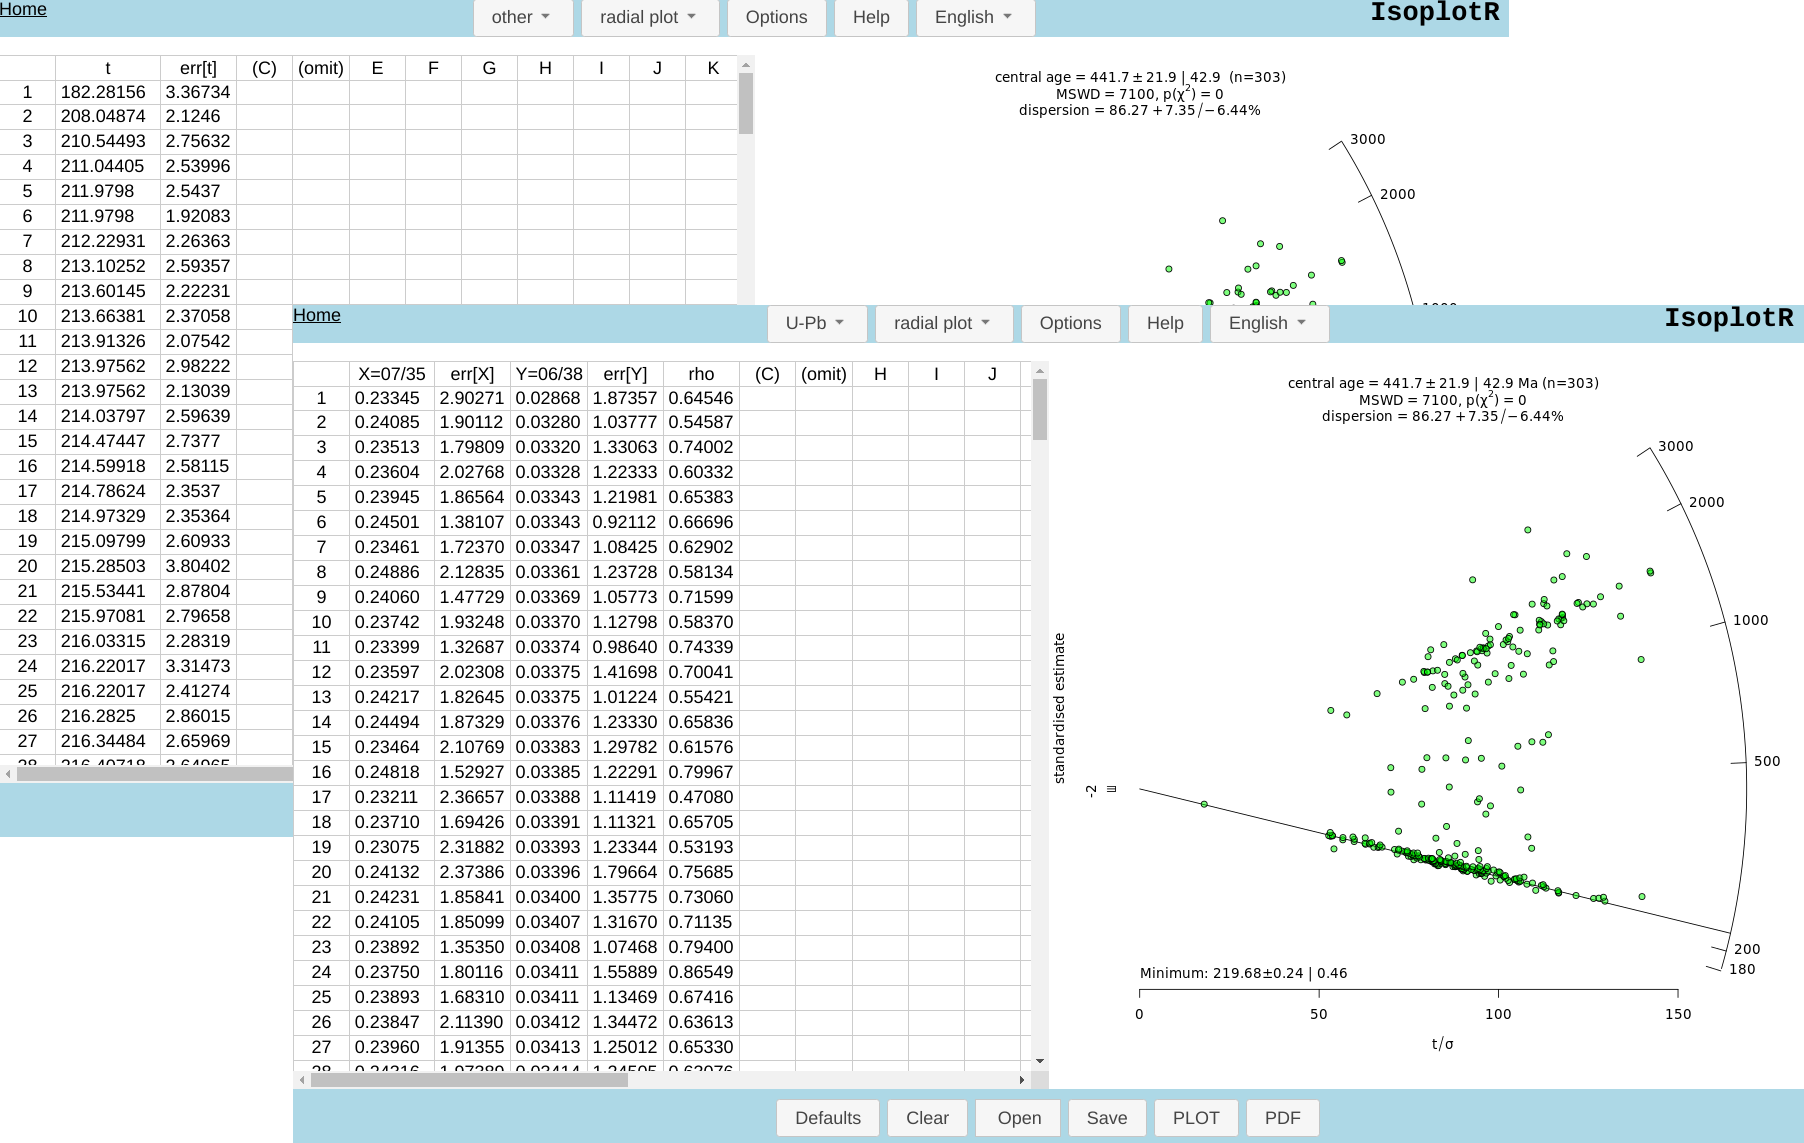
\includegraphics[width=\textwidth]{IsoplotR.png}
  \caption{MLA calculation of LA-ICPMS sample 297 of
    \citet{gehrels2020}, performed using \texttt{IsoplotR}'s graphical
    user interface \citep{vermeesch2018b}. This calculation can either
    be performed from the age estimates (background), or from the
    U--Pb compositions (foreground). Both methods yield identical
    results. }
  \label{fig:IsoplotR}
\end{figure}

\texttt{IsoplotR} is an \texttt{R} package for radiometric
geochronology \citep{vermeesch2018c}. Figure~\ref{fig:IsoplotR} shows
its online user interface. The software implements two ways to plot
radial plots and calculate minimum ages. The first of these is to (1)
select \texttt{other} as a data type, (2) paste the U--Pb ages and
their uncertainties into the input window, (3) choose \texttt{radial
  plot} as an output device, (4) select \texttt{Options} $\rightarrow$
\texttt{Finite mixtures} $\rightarrow$ \texttt{minimum}, and (5) click
\texttt{PLOT}. A second way to use the minimum age model is to (1)
select \texttt{U-Pb} as the data type, (2) paste the U--Pb data into
the input window, (3) proceed as before. Both methods produce
identical results.\\

Alternatively, the same calculations can also be performed from the
command line with the \texttt{R} programming language. Using the ages
and their uncertainties:

\begin{verbatim}
library(IsoplotR)
ages <- read.data("297ages.csv",method="other",
                  format="radial",ierr=1)
radialplot(ages,k="min")
\end{verbatim}

\noindent or using the U--Pb compositions:

\begin{verbatim}
UPb <- read.data("297isotopes.csv",method="U-Pb",
                 format=1,ierr=3)
radialplot(UPb,k="min")
\end{verbatim}

\noindent where \texttt{297ages.csv} and \texttt{297isotopes.csv} are
two comma separated text files with the age data and isotopic
compositions, respectively. These files are provided in the
Supplementary Information. \texttt{297ages.csv} specifies the
uncertainties as absolute values (standard errors), whereas
\texttt{297isotopes.csv} contains relative uncertainties (coefficients
of variation). This difference is handled by the \texttt{ierr}
argument to the \texttt{read.data} function.

%\bibliographystyle{/home/pvermees/Dropbox/abbrvplainnat.bst}
%\bibliography{/home/pvermees/Dropbox/biblio.bib}

\begin{thebibliography}{32}
\providecommand{\natexlab}[1]{#1}
\providecommand{\url}[1]{\texttt{#1}}
\expandafter\ifx\csname urlstyle\endcsname\relax
  \providecommand{\doi}[1]{doi: #1}\else
  \providecommand{\doi}{doi: \begingroup \urlstyle{rm}\Url}\fi

\bibitem[Barbeau et~al.(2009)Barbeau, Olivero, Swanson-Hysell, Zahid, Murray,
  and Gehrels]{barbeau2009}
Barbeau, L., David, Olivero, E.~B., Swanson-Hysell, N.~L., Zahid, K.~M.,
  Murray, K.~E., and Gehrels, G.~E.
\newblock {Detrital-zircon geochronology of the eastern Magallanes foreland
  basin: Implications for Eocene kinematics of the northern Scotia Arc and
  Drake Passage}.
\newblock \emph{Earth and Planetary Science Letters}, 284\penalty0
  (3-4):\penalty0 489--503, 2009.

\bibitem[Chen et~al.(2016)Chen, Huang, Liu, Feng, Chung, and Lee]{chen2016}
Chen, W.-S., Huang, Y.-C., Liu, C.-H., Feng, H.-T., Chung, S.-L., and Lee,
  Y.-H.
\newblock {UPb zircon geochronology constraints on the ages of the Tananao
  Schist Belt and timing of orogenic events in Taiwan: Implications for a new
  tectonic evolution of the South China Block during the Mesozoic}.
\newblock \emph{Tectonophysics}, 686:\penalty0 68--81, 2016.

\bibitem[Cherniak and Watson(2001)]{cherniak2001}
Cherniak, D. and Watson, E.
\newblock Pb diffusion in zircon.
\newblock \emph{Chemical Geology}, 172\penalty0 (1-2):\penalty0 5--24, 2001.

\bibitem[Copeland(2020)]{copeland2020}
Copeland, P.
\newblock On the use of geochronology of detrital grains in determining the
  time of deposition of clastic sedimentary strata.
\newblock \emph{Basin Research}, 2020.
\newblock \doi{10.1111/BRE.12441}.

\bibitem[Coutts et~al.(2019)Coutts, Matthews, and Hubbard]{coutts2019}
Coutts, D.~S., Matthews, W.~A., and Hubbard, S.~M.
\newblock {Assessment of widely used methods to derive depositional ages from
  detrital zircon populations}.
\newblock \emph{Geoscience Frontiers}, 10\penalty0 (4):\penalty0 1421--1435,
  2019.

\bibitem[Dickinson and Gehrels(2009)]{dickinson2009}
Dickinson, W. and Gehrels, G.
\newblock {U-Pb ages of detrital zircons in Jurassic eolian and associated
  sandstones of the Colorado Plateau: Evidence for transcontinental dispersal
  and intraregional recycling of sediment}.
\newblock \emph{Geological Society of America Bulletin}, 121:\penalty0
  408--433, 2009.
\newblock \doi{10.1130/B26406.1}.

\bibitem[Galbraith(1990)]{galbraith1990a}
Galbraith, R.~F.
\newblock The radial plot: graphical assessment of spread in ages.
\newblock \emph{Nuclear Tracks and Radiation Measurements}, 17:\penalty0
  207--214, 1990.

\bibitem[Galbraith and Green(1990)]{galbraith1990b}
Galbraith, R.~F. and Green, P.~F.
\newblock Estimating the component ages in a finite mixture.
\newblock \emph{Nuclear Tracks and Radiation Measurements}, 17:\penalty0
  197--206, 1990.

\bibitem[Galbraith(2005)]{galbraith2005}
Galbraith, R.~F.
\newblock \emph{Statistics for fission track analysis}.
\newblock CRC Press, 2005.

\bibitem[Galbraith(1988)]{galbraith1988}
Galbraith, R.
\newblock Graphical display of estimates having differing standard errors.
\newblock \emph{Technometrics}, 30\penalty0 (3):\penalty0 271--281, 1988.

\bibitem[Galbraith and Laslett(1993)]{galbraith1993}
Galbraith, R. and Laslett, G.
\newblock Statistical models for mixed fission track ages.
\newblock \emph{Nuclear tracks and radiation measurements}, 21\penalty0
  (4):\penalty0 459--470, 1993.

\bibitem[Gehrels(2003)]{gehrels2003}
Gehrels, G.
\newblock {AgePick}, 2003.
\newblock \url{https://sites.google.com/a/laserchron.org/laserchron/home/} Last
  accessed: 2020-06-05.

\bibitem[Gehrels et~al.(2020)Gehrels, Giesler, Olsen, Kent, Marsh, Parker,
  Rasmussen, Mundil, Irmis, Geissman, et~al.]{gehrels2020}
Gehrels, G., Giesler, D., Olsen, P., Kent, D., Marsh, A., Parker, W.,
  Rasmussen, C., Mundil, R., Irmis, R., Geissman, J., et~al.
\newblock {LA-ICPMS U--Pb geochronology of detrital zircon grains from the
  Coconino, Moenkopi, and Chinle Formations in the Petrified Forest National
  Park (Arizona)}.
\newblock \emph{Geochronology}, 2020.

\bibitem[Herriott et~al.(2019)Herriott, Crowley, Schmitz, Wartes, and
  Gillis]{herriott2019}
Herriott, T.~M., Crowley, J.~L., Schmitz, M.~D., Wartes, M.~A., and Gillis,
  R.~J.
\newblock {Exploring the law of detrital zircon: LA-ICP-MS and CA-TIMS
  geochronology of Jurassic forearc strata, Cook Inlet, Alaska, USA}.
\newblock \emph{Geology}, 47\penalty0 (11):\penalty0 1044--1048, 2019.

\bibitem[Keller et~al.(2018)Keller, Schoene, and Samperton]{keller2018}
Keller, C.~B., Schoene, B., and Samperton, K.~M.
\newblock A stochastic sampling approach to zircon eruption age interpretation.
\newblock \emph{Geochemical Perspectives Letters}, 8\penalty0
  (LLNL-JRNL-738859), 2018.

\bibitem[{Ludwig}(1998)]{ludwig1998}
{Ludwig}, K.~R.
\newblock {On the treatment of concordant uranium-lead ages}.
\newblock \emph{Geochimica et Cosmochimica Acta}, 62:\penalty0 665--676, 1998.
\newblock \doi{10.1016/S0016-7037(98)00059-3}.

\bibitem[Ludwig(2003)]{ludwig2003}
Ludwig, K.~R.
\newblock {User's manual for Isoplot 3.00: a geochronological toolkit for
  Microsoft Excel}.
\newblock \emph{Berkeley Geochronology Center Special Publication 4}, 4, 2003.

\bibitem[Ludwig and Mundil(2002)]{ludwig2002}
Ludwig, K. and Mundil, R.
\newblock {Extracting reliable U-Pb ages and errors from complex populations of
  zircons from Phanerozoic tuffs}.
\newblock In \emph{Geochimica et Cosmochimica Acta}, volume~66, pages
  A463--A463, 2002.

\bibitem[Nelson(2001)]{nelson2001}
Nelson, D.~R.
\newblock {An assessment of the determination of depositional ages for
  Precambrian clastic sedimentary rocks by U--Pb dating of detrital zircons}.
\newblock \emph{Sedimentary Geology}, 141:\penalty0 37--60, 2001.

\bibitem[{Nemchin} and {Cawood}(2005)]{nemchin2005}
{Nemchin}, A.~A. and {Cawood}, P.~A.
\newblock {Discordance of the U--Pb system in detrital zircons: Implication for
  provenance studies of sedimentary rocks}.
\newblock \emph{Sedimentary Geology}, 182:\penalty0 143--162, 2005.
\newblock \doi{10.1016/j.sedgeo.2005.07.011}.

\bibitem[Rasmussen et~al.(2020)Rasmussen, Mundil, Irmis, Geisler, Gehrels,
  Olsen, Kent, Lepre, Kinney, Geissman, et~al.]{rasmussen2020}
Rasmussen, C., Mundil, R., Irmis, R.~B., Geisler, D., Gehrels, G.~E., Olsen,
  P.~E., Kent, D.~V., Lepre, C., Kinney, S.~T., Geissman, J.~W., et~al.
\newblock {U-Pb zircon geochronology and depositional age models for the Upper
  Triassic Chinle Formation (Petrified Forest National Park, Arizona, USA):
  Implications for Late Triassic paleoecological and paleoenvironmental
  change}.
\newblock \emph{GSA Bulletin}, 2020.

\bibitem[Ross et~al.(2017)Ross, Ludvigson, M{\"o}ller, Gonzalez, and
  Walker]{ross2017}
Ross, J.~B., Ludvigson, G.~A., M{\"o}ller, A., Gonzalez, L.~A., and Walker, J.
\newblock {Stable isotope paleohydrology and chemostratigraphy of the Albian
  Wayan Formation from the wedge-top depozone, North American Western Interior
  Basin}.
\newblock \emph{Science China Earth Sciences}, 60\penalty0 (1):\penalty0
  44--57, 2017.

\bibitem[{Sambridge} and {Compston}(1994)]{sambridge1994}
{Sambridge}, M.~S. and {Compston}, W.
\newblock {Mixture modeling of multi-component data sets with application to
  ion-probe zircon ages}.
\newblock \emph{Earth and Planetary Science Letters}, 128:\penalty0 373--390,
  1994.
\newblock \doi{10.1016/0012-821X(94)90157-0}.

\bibitem[Titterington and Halliday(1979)]{titterington1979}
Titterington, D.~M. and Halliday, A.~N.
\newblock On the fitting of parallel isochrons and the method of maximum
  likelihood.
\newblock \emph{Chemical Geology}, 26:\penalty0 183--195, 1979.

\bibitem[Tucker et~al.(2013)Tucker, Roberts, Hu, Kemp, and
  Salisbury]{tucker2013}
Tucker, R.~T., Roberts, E.~M., Hu, Y., Kemp, A.~I., and Salisbury, S.~W.
\newblock {Detrital zircon age constraints for the Winton Formation,
  Queensland: contextualizing Australia's Late Cretaceous dinosaur faunas}.
\newblock \emph{Gondwana Research}, 24\penalty0 (2):\penalty0 767--779, 2013.

\bibitem[{van der Touw} et~al.(1997){van der Touw}, Galbraith, and
  Laslett]{touw1997}
{van der Touw}, J., Galbraith, R., and Laslett, G.
\newblock A logistic truncated normal mixture model for overdispersed binomial
  data.
\newblock \emph{Journal of Statistical Computation and Simulation}, 59\penalty0
  (4):\penalty0 349--373, 1997.

\bibitem[Vermeesch(2009)]{vermeesch2009c}
Vermeesch, P.
\newblock {RadialPlotter: A Java application for fission track, luminescence
  and other radial plots}.
\newblock \emph{Radiation Measurements}, 44\penalty0 (4):\penalty0 409--410,
  2009.

\bibitem[Vermeesch(2012)]{vermeesch2012b}
Vermeesch, P.
\newblock On the visualisation of detrital age distributions.
\newblock \emph{Chemical Geology}, 312-313:\penalty0 190--194, 2012.
\newblock \doi{10.1016/j.chemgeo.2012.04.021}.

\bibitem[Vermeesch(2018{\natexlab{a}})]{vermeesch2018b}
Vermeesch, P.
\newblock {Dissimilarity measures in detrital geochronology}.
\newblock \emph{Earth-Science Reviews}, 178:\penalty0 310--321,
  2018{\natexlab{a}}.
\newblock \doi{10.1016/j.earscirev.2017.11.027}.

\bibitem[Vermeesch(2018{\natexlab{b}})]{vermeesch2018c}
Vermeesch, P.
\newblock {\texttt{IsoplotR}: a free and open toolbox for geochronology}.
\newblock \emph{Geoscience Frontiers}, 9:\penalty0 1479--1493,
  2018{\natexlab{b}}.

\bibitem[York et~al.(2004)York, Evensen, Mart\'{i}nez, and
  De~Basabe~Delgado]{york2004}
York, D., Evensen, N.~M., Mart\'{i}nez, M.~L., and De~Basabe~Delgado, J.
\newblock {Unified equations for the slope, intercept, and standard errors of
  the best straight line}.
\newblock \emph{American Journal of Physics}, 72\penalty0 (3):\penalty0
  367--375, 2004.

\bibitem[Zhang et~al.(2016)Zhang, Pease, Skogseid, and
  Wohlgemuth-Ueberwasser]{zhang2016}
Zhang, X., Pease, V., Skogseid, J., and Wohlgemuth-Ueberwasser, C.
\newblock {Reconstruction of tectonic events on the northern Eurasia margin of
  the Arctic, from U-Pb detrital zircon provenance investigations of late
  Paleozoic to Mesozoic sandstones in southern Taimyr Peninsula}.
\newblock \emph{Bulletin}, 128\penalty0 (1-2):\penalty0 29--46, 2016.

\end{thebibliography}

\end{document}
